\documentclass[11pt,a4paper]{article}
\usepackage[utf8]{inputenc}
\usepackage[T1]{fontenc}
\usepackage{lmodern}
\usepackage{microtype}
\usepackage[margin=2.3cm]{geometry}
\usepackage{graphicx}
\usepackage{booktabs}
\usepackage{float}
\usepackage[font=small,labelfont=bf]{caption}
\usepackage{listings}
\usepackage[hidelinks]{hyperref}

\renewcommand{\figurename}{Figura}
\renewcommand{\tablename}{Tabela}
\renewcommand{\contentsname}{Sumário}
\renewcommand{\refname}{Referências}

\lstset{basicstyle=\ttfamily\small, columns=fullflexible,
        frame=single, framerule=0.3pt, backgroundcolor=\color{white}}

\title{Trabalho Prático 2 -- Memória Virtual\\[2pt]
       \large Sistemas Operacionais -- DCC/UFMG}
% TODO: incluir o nome e a matrícula do(a) colega de dupla.
\author{Marcus Vinícius Moraes Oliveira (2022035733), Pedro Dalla-Lana (202420613)}
\date{Novembro de 2026}

\begin{document}
\maketitle

% =====================================================================
\section{Resumo do projeto}

O simulador, escrito em C, lê um \emph{trace} de acessos (endereço
hexadecimal de 32~bits seguido de \texttt{R} ou \texttt{W}), traduz cada
endereço para uma página virtual, consulta a tabela de páginas, trata
as faltas de página com uma política de reposição e conta as páginas
lidas do disco e as páginas sujas escritas de volta. Um trace de um
milhão de acessos é processado em cerca de 0,15~s.

O código tem três módulos. \texttt{main.c} interpreta os argumentos e
encadeia leitura, simulação e relatório; \texttt{ferramentas.c} lê o
trace inteiro para um vetor e traz utilitários de alocação e conversão;
\texttt{simulador.c} é o núcleo, com as tabelas de páginas, os
algoritmos de reposição e o laço de simulação. As tabelas compartilham a
interface \texttt{struct pagetable}, com ponteiros de função
(\texttt{lookup}, \texttt{insert}, \texttt{del}, \texttt{destroy}) e
contadores de memória e de entradas lidas, de modo que o laço não sabe
qual tabela está em uso. Cada quadro físico (\texttt{struct frame})
guarda a página carregada, os bits sujo e referenciado, o instante do
último acesso, a contagem de acessos e os campos auxiliares do LRU e do
LFU; \texttt{struct memory} reúne os quadros e o estado de cada
política. O tempo é um contador incrementado a cada acesso.

O programa é chamado como no enunciado
(\texttt{bin/simulador lru arquivo.log 4 128}) e aceita opções extras:
\texttt{debug} (uma linha por acesso), \texttt{stats} (faltas
compulsórias, custo da tabela e tempo), \texttt{pt=dense|2level|3level|inverted}
e \texttt{seed=N}.

% =====================================================================
\section{Motivação e escolha dos algoritmos}

O Random escolhe a vítima com \texttt{random() \% n} depois
que a memória está cheia. Não usa nenhuma informação do passado e por
isso serve de linha de base: um algoritmo ``inteligente'' precisa
superá-lo para justificar seu custo. A semente é fixa (42).

O LRU remove a página usada há mais tempo, apostando em
localidade temporal. Usa uma lista duplamente encadeada embutida nos
quadros: cada acesso move o quadro para a cabeça e a vítima é a cauda,
ambos em $O(1)$. Mede o valor de conhecer o histórico recente exato.

O LFU remove a página com menos acessos desde que foi
carregada, desempatando pelo acesso mais antigo. Os quadros ficam num
heap mínimo por \texttt{(freq, last\_access)}, com operações em
$O(\log n)$. Representa a hipótese ``o que foi muito usado continuará
sendo''; usamos a versão pura, sem envelhecimento, para observar seus
efeitos colaterais.

O CLOCK, escolhido no critério livre, organiza os quadros em um
círculo; o
ponteiro avança zerando bits de referência ligados (segunda chance) até
achar um desligado, que é a vítima. Um acesso só liga o bit. É a
aproximação de LRU usada em sistemas reais e permite medir quanto se
perde ao trocar o histórico exato por um bit.

Quanto às tabelas de páginas, a densa tem uma entrada por
página virtual ($2^{32-s}$ inteiros). As hierárquicas dividem os
bits da página em 2 (10+10 para 4~KB) ou 3 partes (6+7+7) e alocam
tabelas internas e folhas sob demanda. A invertida tem uma
entrada por quadro físico, localizada por hash multiplicativo com
encadeamento num vetor indexado pelo próprio quadro.

Antes dos experimentos, esperávamos que o LRU vencesse nos programas com
localidade e fosse o pior num laço maior que a memória, onde o Random
deveria ganhar; que o CLOCK ficasse próximo do LRU; e que o LFU se
saísse bem com um conjunto quente estável, mas sofresse com mudanças de
fase. Com mais memória, todos devem convergir para as faltas
compulsórias; com páginas maiores e memória fixa, a perda de quadros
deve superar o ganho de localidade espacial. Entre as tabelas, a densa
deve ser a mais rápida e a mais cara, e a invertida a mais econômica.

% =====================================================================
\section{Decisões de projeto}

Como o tamanho da página chega em KB, $s = 10 + \log_2(\textit{página})$.
\emph{Páginas lidas} contam todas as faltas, inclusive as compulsórias;
\emph{páginas escritas} contam só vítimas sujas, sem escrever as que
sobram no fim. Uma página carregada por \texttt{W} já entra suja.
Quadros livres são sempre usados antes de consultar a política. No LFU
a contagem pertence ao quadro e é zerada quando a página sai. O trace é
lido por inteiro antes da simulação, para que o tempo medido exclua a
E/S, e um mapa de bits marca as páginas já vistas, separando as faltas
compulsórias. Verificamos que os quatro tipos de tabela produzem
exatamente as mesmas faltas e escritas. A corretude foi conferida à mão
com \texttt{testes/pequeno.log} (12 acessos, 4 quadros) no modo
\texttt{debug}.

% =====================================================================
\section{Testes de código}

Além dos logs fornecidos, o script \texttt{testes/gerar\_traces.py}
gera quatro traces de um milhão de acessos cada, com semente fixa, para
isolar comportamentos que os programas reais misturam. Os endereços são
múltiplos de 4 dentro de regiões distintas do espaço de 32 bits.

\begin{table}[H]
\centering\small
\begin{tabular}{@{}lp{9.3cm}l@{}}
\toprule
Trace & Padrão & Objetivo \\
\midrule
\texttt{sequencial} & varre 640~KB (160 páginas de 4~KB) de 64 em 64 bytes, em laço; 30\% escritas & pior caso do LRU \\
\texttt{aleatorio}  & endereços uniformes em 64~MB; 30\% escritas & sem localidade \\
\texttt{localidade} & 80\% dos acessos em 96~KB ``quentes'' (24 páginas), 20\% espalhados em 32~MB & regra 80/20 \\
\texttt{fases}      & 10 fases; em cada uma, 90\% dos acessos em 96~KB de uma região nova, 10\% espalhados & mudança de fase \\
\bottomrule
\end{tabular}
\end{table}

Para regerar: \texttt{python3 testes/gerar\_traces.py}. Os experimentos
completos são reproduzidos por \texttt{python3 experimentos/rodar.py}
(gera os CSVs em \texttt{experimentos/resultados/}, cerca de 5 minutos)
e \texttt{python3 experimentos/graficos.py} (gera as figuras).

% =====================================================================
\section{Análise de desempenho}

Foram usados os traces \texttt{compilador.log} e \texttt{simulador.log}
(um milhão de acessos cada) e os quatro sintéticos. Todos os gráficos
usam escala logarítmica, pois as faltas variam em ordens de grandeza.

\subsection{Variando a memória (páginas de 4 KB)}

\begin{figure}[H]
\centering
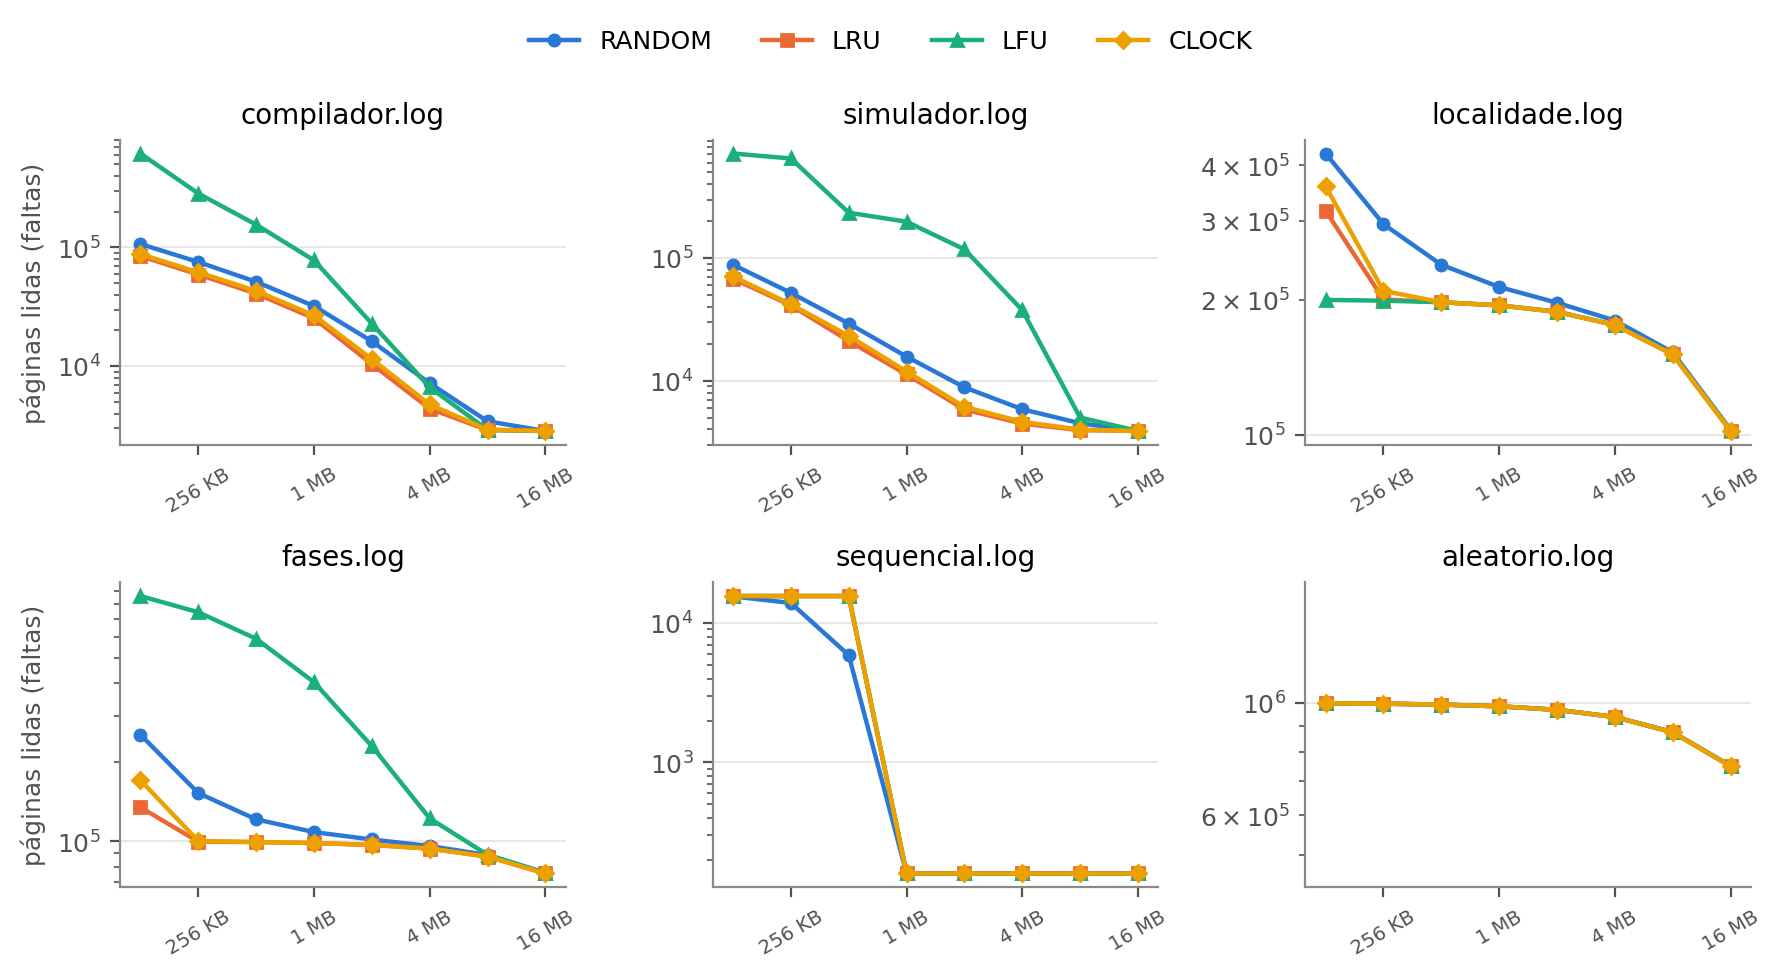
\includegraphics[width=\textwidth]{figuras/faltas_memoria.png}
\caption{Páginas lidas (faltas) em função da memória física, de 128~KB a
16~MB, com páginas de 4~KB.}
\label{fig:mem}
\end{figure}

\begin{table}[H]
\centering\small
\begin{tabular}{@{}lrrrrr@{}}
\toprule
Trace (memória) & Random & LRU & LFU & CLOCK & compulsórias \\
\midrule
compilador (1 MB)   & 32\,062 & 25\,308 & 77\,795 & 26\,789 & 2\,852 \\
simulador (1 MB)    & 15\,715 & 11\,240 & 197\,792 & 11\,876 & 3\,890 \\
localidade (128 KB) & 425\,273 & 316\,629 & 200\,060 & 359\,226 & 8\,216 \\
fases (128 KB)      & 254\,492 & 134\,629 & 857\,979 & 170\,625 & 16\,351 \\
sequencial (512 KB) & 5\,882 & 15\,625 & 15\,625 & 15\,625 & 160 \\
\bottomrule
\end{tabular}
\caption{Páginas lidas em pontos representativos da Figura~\ref{fig:mem}.}
\label{tab:mem}
\end{table}

No compilador e no simulador o LRU é o melhor em toda a faixa, e o
CLOCK fica de 2\% a 10\% acima dele --- o preço de usar um bit em vez da
ordem exata. O Random paga de 25\% a 65\% a mais com até 4~MB, o que
mostra que esses programas têm localidade temporal real: saber o
passado recente vale bastante. A partir de 8--16~MB o conjunto de
trabalho inteiro cabe na memória (2\,852 e 3\,890 páginas distintas,
isto é, 11 e 15~MB) e todos os algoritmos convergem para as faltas
compulsórias.

O resultado mais marcante é o LFU: 3 vezes pior que o LRU no compilador
e 17 vezes pior no simulador com 1~MB, pior até que o Random. A causa é
a \emph{poluição por frequência}: páginas usadas intensamente no início
da execução acumulam contadores enormes e nunca mais saem, ocupando
quadros que o programa já não usa. Sobra para as páginas atuais uma
fração pequena da memória, onde cada página nova entra com
\texttt{freq = 1} e é a próxima vítima --- o algoritmo passa a se
comportar como uma memória minúscula. O trace \texttt{fases} reproduz
isso de forma controlada (LFU com 6 vezes mais faltas que o LRU em
128~KB): o conjunto quente de cada fase acumula contagens que impedem a
entrada do conjunto da fase seguinte. O efeito só some quando a memória
comporta tudo (16~MB).

No trace \texttt{localidade} com 128~KB (32 quadros para 24 páginas
quentes), o LFU tem 37\% menos faltas que o LRU. Ali 20\% dos acessos
são a páginas de uso único; no LRU cada uma delas vira a mais recente e
empurra uma página quente para fora, enquanto no LFU elas entram com
contagem 1 e saem sem incomodar as quentes. Assim que sobra espaço
(256~KB), os quatro algoritmos se igualam, porque as faltas restantes
são as dos acessos espalhados, que nenhum algoritmo evita.

No laço \texttt{sequencial} de 160 páginas, com 32 a 128 quadros, LRU,
LFU e CLOCK erram \emph{toda} troca de página (15\,625 faltas =
$10^6 \times 64 / 4096$): a página expulsa é sempre a próxima a ser
usada. O Random, por não seguir o padrão, mantém por acaso parte do
laço na memória e tem 2,7 vezes menos faltas com 512~KB. É o caso
clássico em que a hipótese de localidade temporal do LRU falha. Com
1~MB o laço cabe inteiro e só restam as 160 faltas compulsórias.

No trace \texttt{aleatorio} os quatro algoritmos são indistinguíveis
(diferença $<0{,}3\%$): a taxa de faltas é simplesmente
$1 - \textit{memória}/\textit{espaço usado}$.

Repetimos o Random com 10 sementes para cada ponto da
Figura~\ref{fig:mem}. O desvio padrão ficou sempre abaixo de 0,6\% da
média (por exemplo, compilador com 1~MB: $31\,972 \pm 75$), então uma
única semente é representativa e as diferenças acima não são ruído.

\subsection{Páginas escritas}

\begin{figure}[H]
\centering
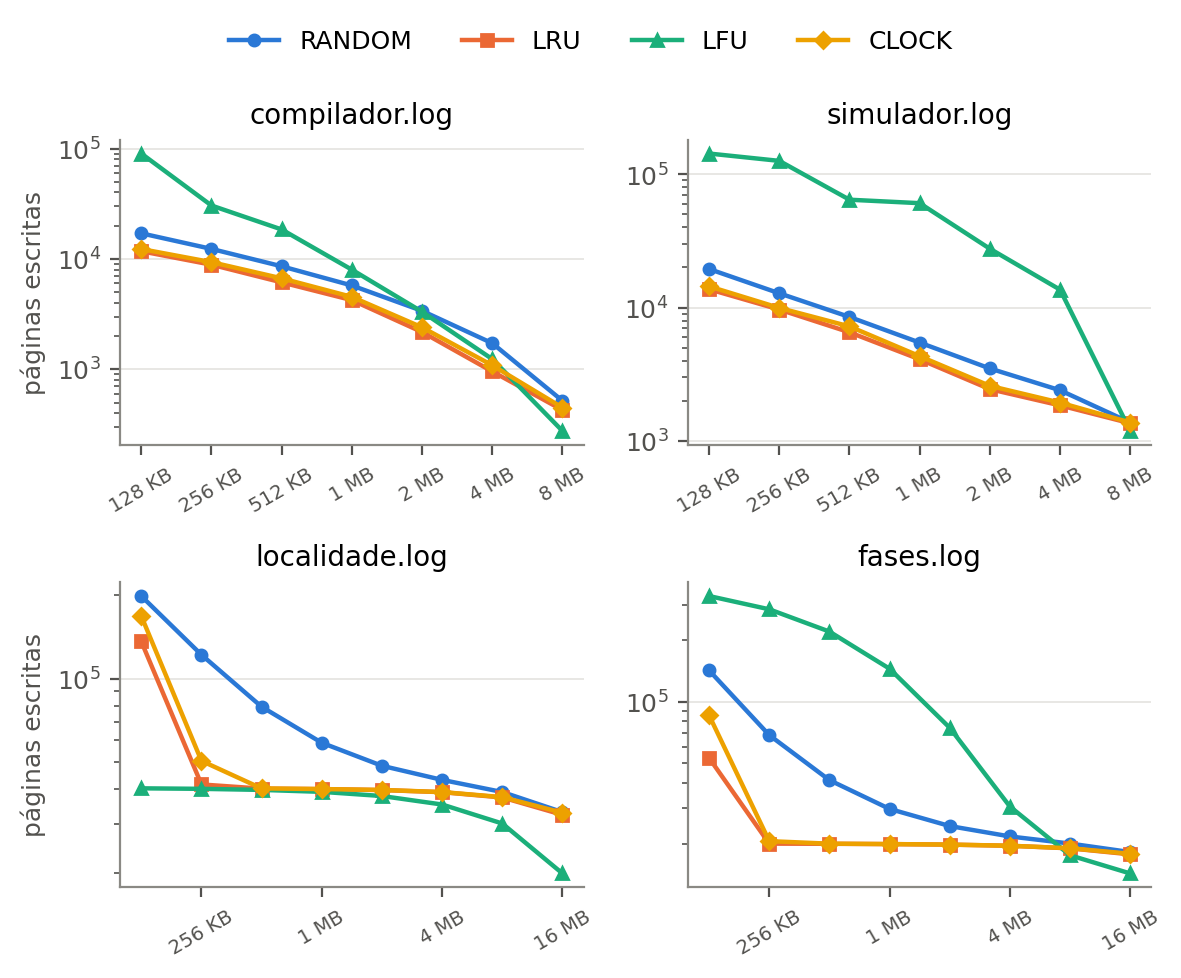
\includegraphics[width=0.75\textwidth]{figuras/escritas_memoria.png}
\caption{Páginas sujas escritas no disco em função da memória (páginas
de 4~KB). Com 16~MB não há nenhuma escrita (ponto omitido na escala
logarítmica).}
\label{fig:esc}
\end{figure}

As escritas seguem as faltas: só há escrita quando há substituição.
Nos programas reais elas representam de 14\% a 42\% das páginas lidas com
LRU e CLOCK (a fração cresce com a memória, pois as poucas páginas
expulsas tendem a ser as que foram modificadas), e caem a zero com 16~MB (nada é expulso). O LFU, além de
ler mais, escreve mais na maior parte da faixa, pelo mesmo motivo. O caso interessante é o
\texttt{localidade}: com memória suficiente o LFU tem o mesmo número de
faltas que os outros, mas até 38\% menos escritas, porque as páginas
mais acessadas --- que concentram as escritas --- nunca são escolhidas
como vítima; quem sai são as de uso único, em geral limpas. Nenhum dos
algoritmos implementados considera o bit sujo na escolha da vítima; uma
variante do CLOCK que prefira páginas limpas (como o NRU ou o
WSClock) reduziria esse custo.

\subsection{Variando o tamanho da página (memória de 1 MB)}

\begin{figure}[H]
\centering
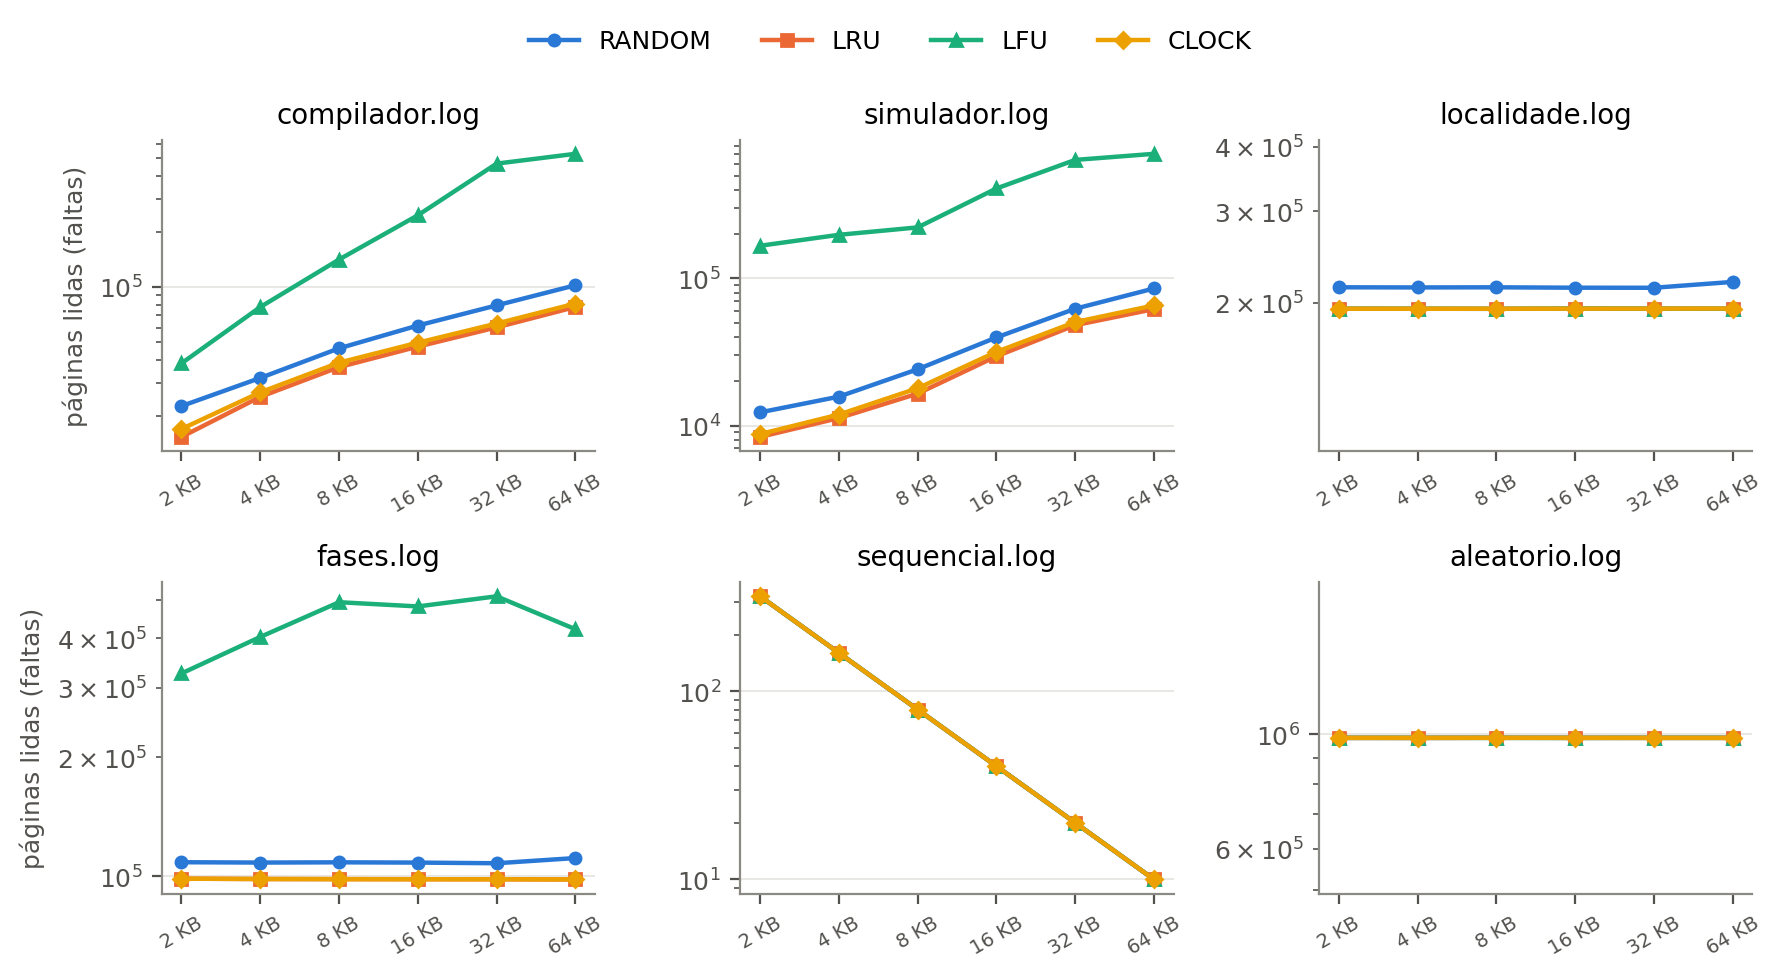
\includegraphics[width=\textwidth]{figuras/faltas_pagina.png}
\caption{Páginas lidas em função do tamanho da página, de 2~KB a 64~KB,
com memória física fixa de 1~MB (de 512 a 16 quadros).}
\label{fig:pag}
\end{figure}

Com a memória fixa, dobrar a página divide o número de quadros por dois.
A localidade espacial reduz as faltas compulsórias (compilador: de
3\,621 páginas distintas com 2~KB para 1\,260 com 64~KB), mas a memória
passa a comportar menos regiões distintas (só 16 com 64~KB).
Nos programas reais o segundo efeito domina com folga: com LRU, as
faltas crescem 5 vezes no compilador (15\,330 $\to$ 77\,837) e 7 vezes
no simulador (8\,364 $\to$ 61\,829) de 2~KB para 64~KB. Esses programas
acessam muitas estruturas pequenas espalhadas pelo espaço de endereços,
e uma página grande carrega muitos bytes que não serão usados. E como
cada falta transfere uma página maior, o volume de dados lidos do disco
cresce ainda mais rápido que o número de faltas.

O \texttt{sequencial} é o oposto: os acessos são contíguos, então só a
localidade espacial importa, e as faltas caem pela metade a cada
duplicação da página (320 $\to$ 10). No \texttt{aleatorio} e no
\texttt{localidade} a curva é plana, porque a fração do espaço que cabe
na memória não depende do tamanho da página. A ordem entre algoritmos
não muda: LRU $\le$ CLOCK $<$ Random nos reais, e o LFU continua
péssimo (de 2,5 a 20 vezes o LRU), com oscilações porque a poluição
depende de quais regiões ficam ``presas'' em cada granularidade.

\subsection{Tabelas de páginas}

O tipo de tabela não muda nenhuma falta; muda o custo de memória da
estrutura e o custo de cada consulta.

\begin{figure}[H]
\centering
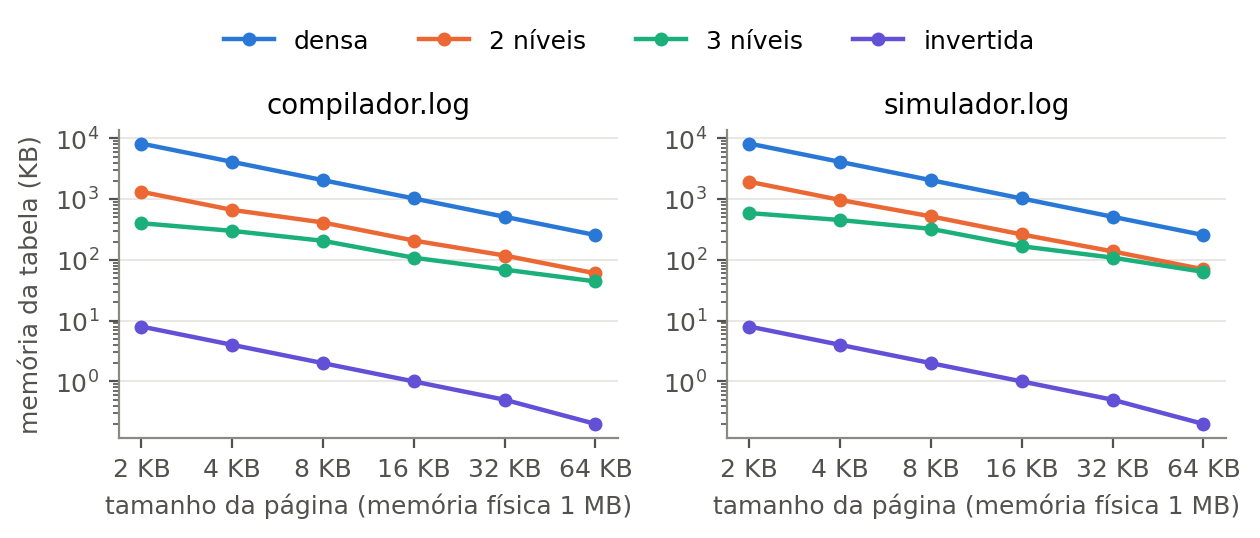
\includegraphics[width=0.85\textwidth]{figuras/tabela_memoria.png}
\caption{Memória ocupada pela tabela de páginas em função do tamanho da
página (memória física de 1~MB).}
\label{fig:pt}
\end{figure}

\begin{table}[H]
\centering\small
\begin{tabular}{@{}llrrrr@{}}
\toprule
Trace & Tabela & Memória & Tabelas alocadas & Entradas lidas/consulta & Tempo (ms) \\
\midrule
compilador & densa     & 4\,096 KB & 1   & 1,00 & 13 \\
           & 2 níveis  &   664 KB & 165 & 2,00 & 15 \\
           & 3 níveis  &   300 KB & 579 & 3,00 & 17 \\
           & invertida &     4 KB & 1   & 2,33 & 17 \\
\midrule
aleatorio  & densa     & 4\,096 KB & 1   & 1,00 & 20 \\
           & 2 níveis  &    72 KB & 17  & 2,00 & 22 \\
           & 3 níveis  &  65,5 KB & 130 & 3,00 & 31 \\
           & invertida &     4 KB & 1   & 1,50 & 36 \\
\bottomrule
\end{tabular}
\caption{Custo das tabelas com páginas de 4~KB e memória de 1~MB
(LRU, um milhão de acessos). O tempo é o do laço de simulação inteiro,
menor de 5 execuções.}
\label{tab:pt}
\end{table}

Em memória, a tabela densa custa $4 \cdot 2^{32-s}$ bytes
independentemente do programa: 8~MB com páginas de 2~KB, 4~MB com
4~KB. As hierárquicas só alocam folhas para as regiões tocadas: o
compilador usa 164 folhas de 4~KB na tabela de 2 níveis (664~KB, 6
vezes menos que a densa) e a de 3 níveis, com folhas menores, desce a
300~KB. A vantagem do terceiro nível encolhe com páginas grandes (o
espaço virtual já é pequeno) e o ganho é maior quanto mais esparso o
uso: o \texttt{aleatorio}, concentrado em 64~MB, precisa de só 16
folhas. A invertida custa proporcionalmente à memória \emph{física}
(256 quadros $\to$ 4~KB) --- três ordens de grandeza abaixo das demais
e independente de quão espalhado é o programa.

Quanto ao tempo de consulta, a densa resolve tudo com uma leitura; a
de 2 níveis com duas e a de 3 níveis com três (menos quando o
diretório intermediário ainda não existe). A invertida lê o balde e
percorre a cadeia: com fator de carga 0,5 a média foi de 2,2 a 2,5
leituras nos programas reais e 1,5 no \texttt{aleatorio},
onde quase toda consulta é uma falta que termina num balde vazio ou
curto. Em tempo absoluto, o laço completo de simulação fica entre 13 e 36~ns por
acesso, com a densa sempre mais rápida. As diferenças são pequenas
porque a simulação inteira cabe no cache; no \texttt{aleatorio}, sem
localidade, as hierárquicas e a invertida perdem mais, pois cada nível
extra é um acesso fora do cache. A invertida tem ainda um custo que não
aparece aqui: localizar uma página exige o hash e não há como
compartilhar a tabela entre processos sem incluir o identificador do
processo na chave.

% =====================================================================
\section{Conclusão}

As hipóteses se confirmaram em quase todos os pontos. O LRU foi o
melhor algoritmo nos programas reais e o CLOCK ficou a menos de 10\%
dele com custo $O(1)$ e um bit por quadro, o que justifica seu uso em
sistemas reais. O Random ficou 25--65\% pior onde há localidade, mas
venceu com folga no laço sequencial, o caso patológico do LRU, e mostrou
variação desprezível entre sementes. Aumentar a memória faz todos
convergirem para as faltas compulsórias; aumentar a página com memória
fixa piorou os programas reais, porque a perda de quadros superou o
ganho de localidade espacial.

A divergência principal foi o tamanho do fracasso do LFU. Esperávamos
que ele perdesse em mudanças de fase, mas não que fosse até 17 vezes pior
que o LRU e pior que o Random nos dois programas reais. A causa é que o
LFU puro nunca esquece: contagens acumuladas em fases antigas prendem
quadros indefinidamente. Ele só se destacou no cenário 80/20 com
memória justa, em que protege as páginas quentes dos acessos de uso
único, e por escrever menos páginas no disco.

Para as tabelas de páginas, a densa é a mais rápida mas desperdiça
megabytes num espaço de 32 bits; a hierárquica é o meio-termo usado na
prática; e a invertida é imbatível em memória, ao custo de uma busca por
hash e de uma ou duas leituras extras por consulta.

Como trabalhos futuros, sugerimos (i) LFU com envelhecimento (dividir os
contadores periodicamente) ou algoritmos híbridos como LRU-K/ARC, que
combinam recência e frequência e evitariam a poluição observada;
(ii) políticas que prefiram vítimas limpas para reduzir escritas;
(iii) simular uma TLB para que a diferença entre as tabelas apareça
como na prática; (iv) medir o tempo das tabelas com contadores de
hardware, já que as diferenças de alguns nanossegundos estão perto do
ruído de medição.

\section{Uso de LLM}
LLM foi utilizada para auxílio na depuração do código, organização do relatório, e transcrição para o formato latex. Além de ter gerado o código base para o arquivo da análise experimental; todo o código foi validado manualmente

\end{document}